%Dokumentinnstillinger:---------------------------------
%Ved å google flitting kan du finne ut hva de forskjellige tingene her betyr, og hvordan du kan gjøre eventuelle endringer.
\documentclass[a4paper,11pt,norsk]{article}
\usepackage[utf8]{inputenc}
\usepackage{a4wide}
\usepackage{lmodern}
\usepackage[T1]{fontenc}
\usepackage{babel}

\setlength{\parindent}{0pt} 
\setlength{\parskip}{2ex}
\usepackage{fixltx2e}
\usepackage{amsmath}
\usepackage[pdftex, pdfborderstyle={/S/U/W 0}]{hyperref}
\usepackage{graphicx}
\usepackage[font=small,labelfont=bf]{caption}
\usepackage{tabularx}
\usepackage{multirow}
\usepackage{circuitikz}
% Adds seperation between two elements with a comma. Format: "    ,    ".
\newcommand{\comma}{\quad , \quad}
% Gives double underline under selected text.
\def\dunderline#1{\underline{\underline{#1}}}
% Faster way to make an equation that can be formatted with "&" to look nice.
\def\spliteq#1{\begin{equation}\begin{split}{#1}\end{split}\end{equation}\\}
%------------------------------------- End -------------------------------------

\begin{document}

%Headingdel:---------------------------------------------
\begin{minipage}[c]{0.15\textwidth}

\includegraphics[width=2.0cm]{Design_projects/elsys_pos_staaende_ntnu.png}
\end{minipage}
\begin{minipage}[c]{0.85\textwidth}

\renewcommand{\arraystretch}{1.7}
\large 
\begin{tabularx}{\textwidth}{|X|X|}
\hline
\multicolumn{2}{|l|}{} \\
\multicolumn{2}{|l|}{\huge \textbf{Designnotat 1}} \\
\multicolumn{2}{|l|}{}  \\
\hline
\multicolumn{2}{|l|}{Tittel: 
%Skriv inn tittel her:------------------------------------------
Variabel Nivåregulator (dempeledd)
} \\
\hline
\multicolumn{2}{|l|}{Forfattere: 
%Skriv inn forfattere her:--------------------------------------
Sindre Danielsen
} \\
\hline
%Skriv inn versjon og dato her her:-----------------------------
Versjon: 3.0 & Dato: 29.05.21
\\
\hline 
\end{tabularx}
\end{minipage}
\normalsize

%Automatisk generert innholdsfortegnelse:------------------

\setlength{\parskip}{0ex}
\renewcommand{\baselinestretch}{0.1}\normalsize
\tableofcontents
\renewcommand{\baselinestretch}{1.00}\normalsize
\setlength{\parskip}{2ex}
\rule{\textwidth}{1pt}

%Selve rapporten:----------------------------------------÷
\newpage
\section{Problembeskrivelse}
\label{sec:innledning}
Vi skal her ta for oss hvordan demping av signaler i et elektronisk system kan konstrueres. Dette ved bruk av en nivåregulator vist i figur~\ref{fig:gnRegulator}. \\
\begin{figure}[htbp]
    \centering
    \begin{circuitikz} [american voltages, european resistors, baseline=(current bounding box.center)]
        \ctikzset { label/align = straight }
        \draw (0,2)
        to [V, l=$V_0$] (0,0);
        \draw (0,2)
        % Top-left side
        to[R=$R_{k}$] (2.5,2)
        to[short,i=$I$, -o] (4,2)
        to[short] (4.5,2)
        (4, 1.6) to [open,v=$v_1$] (4,0.4)
        % Bottom-left side
        (0,0) to[short, -o] (4,0)
        to[short] (4.5,0)
        % Top-right side
        (8.5,2) to[short, -o] (9,2)
        to[short] (11, 2)
        to[R=$R_L$] (11, 0)
        (9, 1.6) to [open,v=$v_2$] (9,0.4)
        % Bottom-right side
        (11, 0) to[short, -o] (9,0)
        to[short] (8.5,0)
        
        % Kilde text
        (0,-0.9) node[below] {Kilde}
        % Last text
        (11,-0.9) node[below] {Last}
        ;
        % Left dashed box
        \node[draw,dashed,minimum width=3.2cm,minimum height=3.8cm,anchor=south west] at (-0.75,-0.90);
        % Right dashed box
        \node[draw,dashed,minimum width=2.5cm,minimum height=3.8cm,anchor=south west] at (10,-0.90);
        % Nivåregulator
        \node[draw,minimum width=4cm,minimum height=3.8cm,anchor=south west] at (4.5,-0.90){Nivåregulator};

        
    \end{circuitikz}
    \caption{Generelt oppsett av en nivåregulator \cite{gn}}
  \label{fig:gnRegulator}
\end{figure}
\\
Nivåregulatoren tar inn et signal $v_1$ definert fra kilden og utvikler et utgangssignal $v_2$, som går gjennom lasten $R_L \approx \infty$. For et slikt system ønsker vi til enhver tid at $v_2 \leq v_1$, slik at det må finnes en amplitude $A$, slik at:
\begin{equation}\label{eq: amplitude}
    v_2(t) = Av_1(t) \comma A\in\left[0,1\right]
\end{equation}\label{eq:reduceV}\\
Kravet for et slikt system er at $\Delta A < 0.1$dB (amplitudeforskjellen mellom den teoretiske modellen og den praktiske gjennomføringen).
\\\\
Annen informasjon fra figur~\ref{fig:gnRegulator}: \\
- $R_k$ er kildens indre motstand, og $V_0$ er spenningsforsyningens signalstyrke. \\
- $I$ er strømretningen.

\newpage
\section{Prinsipiell løsning}
\label{sec:prinsipielllosning}
Kretsdesignet til nivåregulatoren er vist i figur~\ref{fig:krets}. \\
\begin{figure}[htbp]
    \centering
    \begin{circuitikz} [american voltages, european resistors, european vresistors, baseline=(current bounding box.center)]
        \ctikzset { label/align = straight }
        \draw (0,0)
        to[short, o-] (2.5,0)
        to[R=$R_1$] (2.5, -2);
        \draw (2.5, -2)
        to[pR,  pR=$R$] (2.5, -4)
        ;
        \draw(2.5, -4)
        to[R=$R_2$] (2.5, -6)
        (2.75,-7) node[below] {Nivåregulatoren}
        (0, -2.5) to[open, v=$v_1$] (0,-3.5)
        (6, -4.5) to[open, v=$v_2$] (6,-5.5)
        ;
        \draw (2.5,-4) to[short, -o](6, -4)
        ;
        \draw (0,-6) to[short, o-o] (6,-6)
        ;
        \node[draw,dashed,minimum width=3.5cm,minimum height=8cm,anchor=south west] at (1,-7);
        
        
    \end{circuitikz}
    \caption{Kretsen til nivåregulatoren \cite{krets}}
    \label{fig:krets}
\end{figure} \\
Kretsen er en mulig løsning på en nivåregulator. Skal den fungere som et dempeledd, som holder signalstyrken mellom to nivåer mindre eller lik $v_1$, så har vi at: \\ $A \in [A_1, A_2]$, der $0 \leq A \leq 1$.
Minimums- og maksimums-verdien til potensiometeret $R$ \\bestemmer  motstandene $R_1$ og $R_2$. Matematisk er dette fremlagt i vedlegg~\ref{attach:resistors}, som medfører at:\\
\begin{equation}\label{eq: resistors}
    R_1 = \frac{R_2(1-A_1)}{A_1} \comma
    R_2 = \frac{A_1A_2R_{max}}{A_1-A_2}
\end{equation} \\
der $R_{max}$ er den største verdien $R$ kan ha.
\\
\newpage
\section{Realisering og test}
\label{sec:realisering}
Ved realiseringen av kretsen, så velges verdiene vist i tabell~\ref{table:variabler}.
\\
\begin{table}[htbp]
\centering
\begin{tabular}{ |c|c|c|c| } 
\hline
\textbf{Navn} & \textbf{Verdi} & \textbf{Beskrivelse} \\
\hline
$A_1$ & $0.355 \: (-9$dB$)$ & Valgt nedre amplitude.\\
\hline
$A_2$ & $0.014 \: (-37$dB$)$ & Valgt øvre amplitude.\\
\hline
$R_{max}$ & $10$k$\Omega$ &  Valgt potensiometer. \\ 
\hline
$R_1$ & $267\Omega$ & Gitt av likning~\ref{eq: resistors}. \\ 
\hline
$R_2$ & $147\Omega$ & Gitt av likning~\ref{eq: resistors}.\\
\hline
$V$ & $4.780$V & Valgt spenningskilde. \\
\hline
$v_{A_1}$ & $1.697$V & Gitt av likning~\ref{eq:reduceV} ($v_1 = V$). \\
\hline
$v_{A_2}$ & $0.067$V & Gitt av likning~\ref{eq:reduceV} ($v_1 = V$). \\
\hline
\end{tabular}
\caption{Verdiene brukt i realisering av systemet.}
\label{table:variabler}
\end{table}
\\
Den oppkoblede kretsen er vist i figur~\ref{fig:realKrets}.

\begin{figure}[htbp]
    \centering
    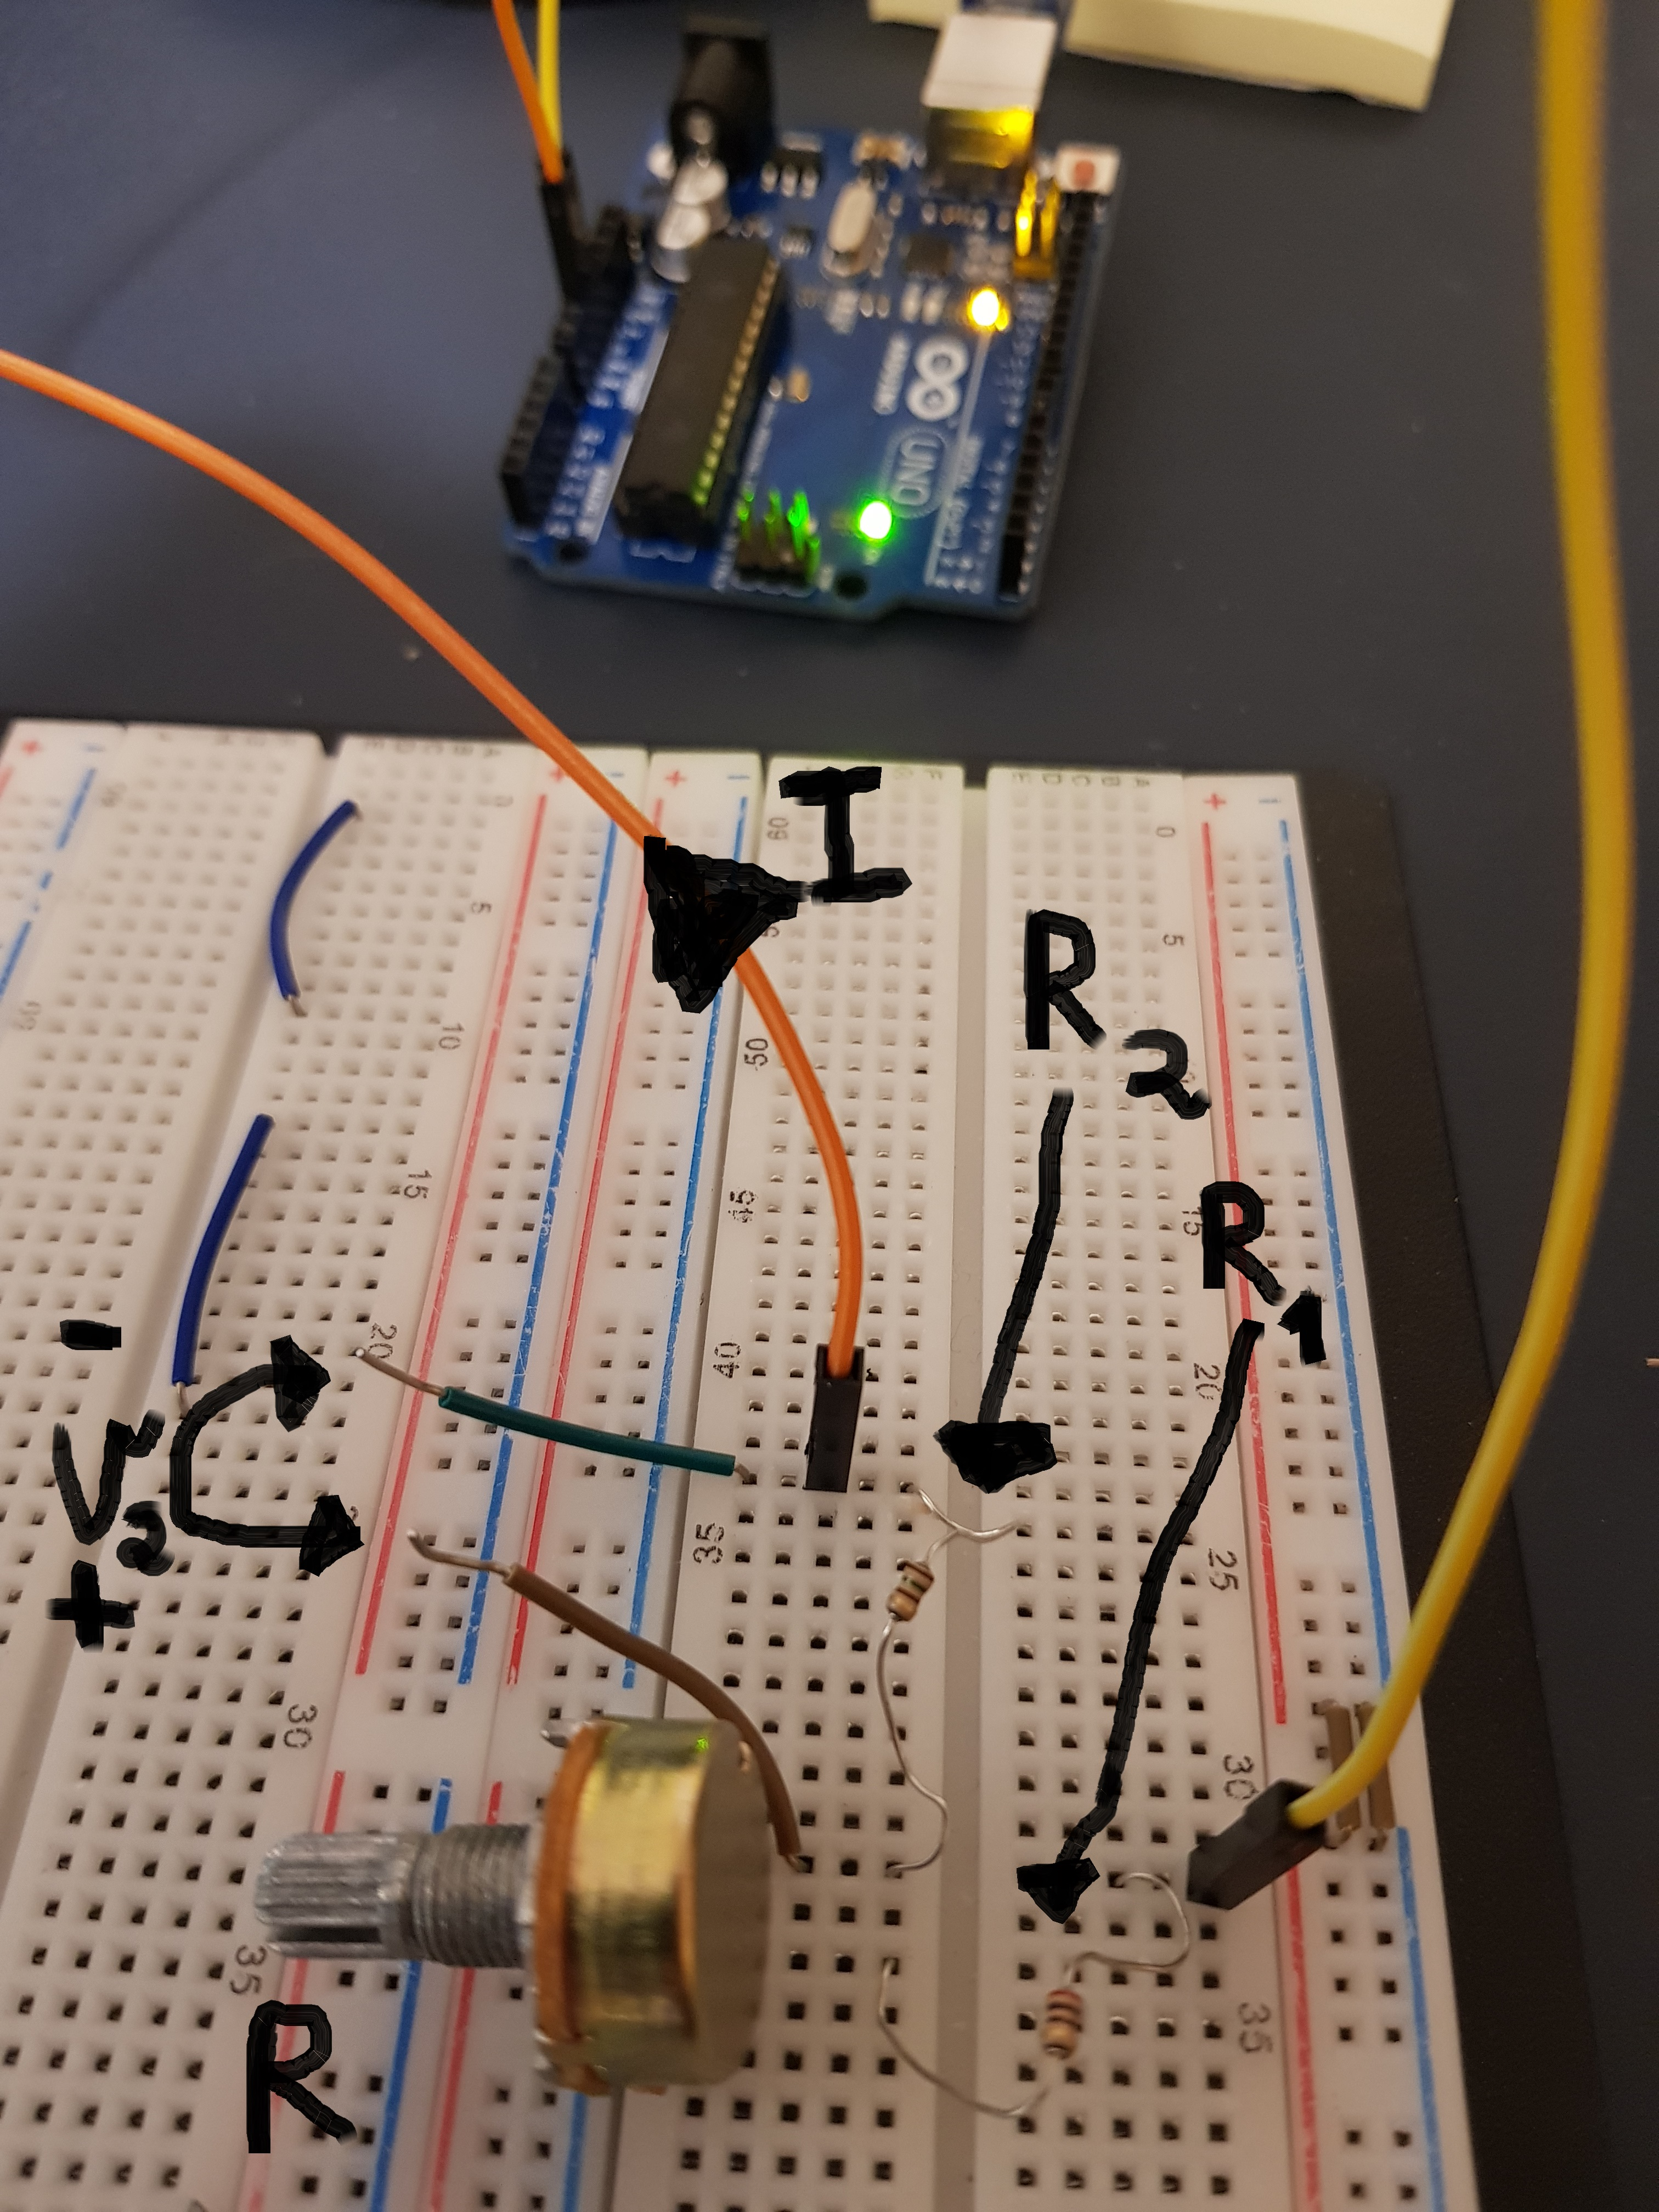
\includegraphics[width=0.6\textwidth]{img/realKrets}
    \caption{Reell krets av figur~\ref{fig:krets}}.
    \label{fig:realKrets}
\end{figure}


\newpage
Det gjøres målinger av spenningsfallet over $R_2$, ved forskjellige verdier av $R$. Oppførselen er vist på grafen til figur~\ref{fig:graph}.
\begin{figure}[htbp]
    \centering
    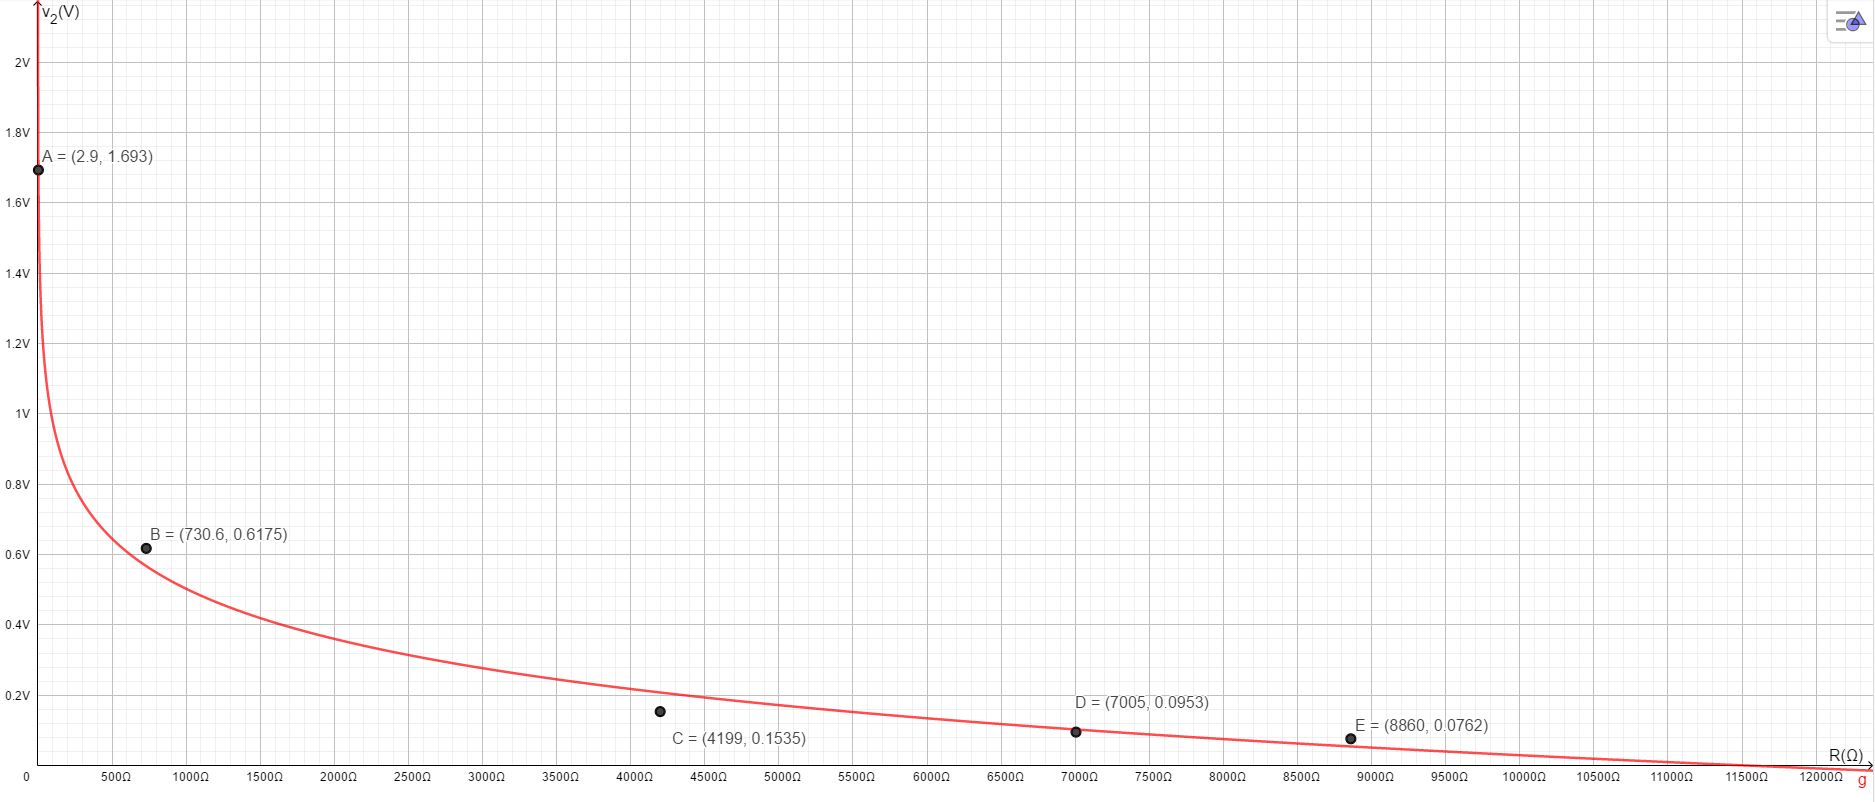
\includegraphics[width=1\textwidth]{img/graph}
    \caption{Oppførselen til $v_2$ når $R$ endres.}
    \label{fig:graph}
\end{figure}

Det første som er verdt å merke er at potensiometeret $R$ ikke kan nå  0$\mathrm{\Omega}$, men stopper ved 2,9$\mathrm{\Omega}$ og at den største målte verdien kun er 8,8k$\mathrm{\Omega}$. Dette vil gi avvik fra likning~\ref{eq: resistors}, der avviket til $v_{A_1} = 39$mV og $v_{A_2} = 8,8$mV.
For å finne ut om avviket har en betydning for $A_1$ og $A_2$, så kan vi bruke likning~\ref{eq: amplitude} og konvertere til dB:
\spliteq {
   & A_{avvik 1} = -9dB - 20\cdot\log_{10}{\left(\frac{1.693\textrm{V}}{4.78\textrm{V}}\right)} = 0.015dB  \\
   & A_{avvik 2} = -37dB - 20\cdot\log_{10}{\left(\frac{0.0762\textrm{V}}{4.78\textrm{V}}\right)} = 1.050dB
}
 Verken $A_1$ eller $A_2$ er innenfor det gitte toleranseområdet fra seksjon~\ref{sec:innledning} på $0.1$dB. En av årsakene til dette er at motstandene brukt i testingen har et avvik på $R_t\in\pm[0\mathrm{\Omega},\:5\mathrm{\Omega}]$ fra motstandene som ble regnet ut i likning~\ref{eq: resistors}. \\
Det er også mulig å se på grafen fra figur~\ref{fig:graph}, at de målte punktene ikke ligger på den forventede funksjonen. De ligger litt i underkant eller overkant.
\\
Merk at kabler inneholder en indre motstand, samt at systemet mister energi i form av varme, som kan påvirke resultatet.

\newpage
\section{Konklusjon}
\label{sec:konklusjon}
Det er brukt en av flere mulige metoder for å utvikle en nivåregulator for dempe et inngangssignal. Målet var å kunne dempe signalet innenfor et variabelt område med en toleranse på $0.1$dB. Etter realiseringen av nivåregulatoren, så kom det frem at avviket ble større en godkjent toleranse, som blant annet skyldes at de realistiske komponentene ikke er nærme nok til de teoretiske beregningene. Skal resultatet forbedres, så må det eventuelt velges andre nedre- og øvre-grenser på $A$ eller bruke realistiske motstander med verdier nærmere den teoretiske modellen.
\newpage

\begin{thebibliography}{9}

\bibitem{gn}
L. Lundheim: En generell nivåregulator \\
\textit{Teknisk notat 1, 2017}, Blackboard.
\bibitem{krets}
Lars Lundheim: Krets a) nivåregulator \\
\textit{Teknisk notat 1, 2017}, Blackboard.
\end{thebibliography}

\section{Vurdering av teksten}
\subsection{Generelt}
\begin{itemize}
    \item Notatet gir en god innsikt i hva som skal utvikles.
    \item Det trekker også med presis formulering av hvordan en generell nivåregulator fungerer.
    \item Den røde tråden i teksten ser ut til å være dempingsvariabelen A, som blir deklarert og formulert og sammenliknet med testresultatene.
    \item Variabler, likninger og figurer blir forklart slik at det vesenetlige kommer med, men fremdeles presist.
    \item Språket virker å være for det meste nøytralt, der "vi" brukes ofte.
    \item Det ser her ut til at det blir kun nevnt relevant stoff for å forstå figurere, likninger og konsepter. 
    \item Utstyret brukt er standard utstyr for en elektronisk utvikler, slik at det er lett anskaffelig. Men de plotte målingene kan være vanskelig å få helt like, i og med at et potensiometer er følsomt for berøring.
    \item Målingene bruker teorien satt opp under seksjon 2 om prinsipiell løsning, samt prøver å forklare hvorfor et større avvik enn ønsket oppstår.
    \item Teksten er relevant og situasjonen til forfatteren blir ikke beskrevet.
\end{itemize}

\subsection{Teknikaliteter}
\begin{itemize}
    \item Variabler er i kursiv og deres hensikt blir forklart.
    \item Figurer viser nok informasjon til at en leser skal sammen med tekst forstå hva den inneholder. 
    \item Likninger er presise, nummerert, og fremgangsmåten fra generelle prinsipp til den spesielle formelen for $R_1$ og $R_2$ blir forklart på en god måte.
    \item Realisert krets viser helheten av kretsen, samt hvilken variabel som tilhører hver komponent.
    \item Figurer blir tallfestet og har presis figurtekst.
    \item Figurer blir referert til i teksten når variabler og konsepter forklares.
    \item Enheter er brukt og er ikke i kursiv, men variabler er i kursiv.
\end{itemize}



\subsection{Kilder}
\begin{itemize}
    \item Kildene har et forståelig oppsett og blir brukt der de har behov for det. Nummereringen er også grei.
\end{itemize}

\subsection{Ønsker tilbakemelding på}
\begin{itemize}
    \item Er det nødvendig å ha med alternative løsninger eller nevne dem?
    \item At jeg definerer nivåregulatoren med en formel i problembeskrivelsen og setter kravet for systemet, er det riktig å gjøre det i problembeskrivelsen?
    \item Er det noen mangler ved problembeskrivelsen?
    \item Eks. potensiometeret mitt viser at det er 10 kilo ohm, men når jeg måler den er den på 8,8 kilo ohm. Hva skal jeg egentlig gå ut ifra når jeg gjør mine beregninger? Målingene på komponentene eller det som de "skal" ha av verdi?
\end{itemize}
\newpage
%Bibliografi: Legg til flere elementer ved å legge til flere \bibitem:--------
\phantomsection

\appendix
%Tillegg. Flere tillegg legges til ved å lage flere sections:-----------------
\section{Utledning av $R_1$ og $R_2$}\label{attach:resistors}

Fra likning~\ref{eq: amplitude}, så har vi at:
\spliteq {
    A = \frac{v_2}{v_1}
}
Fra figur~\ref{fig:krets}, som viser seriekobling av motstandene $R_1, R_2$ og $R$, så kan vi skrive det som:
\spliteq {
    A = \frac{R_2}{R_1 + R  + R_2}
}

Siden minimumsamplituden $A_1 \implies R \approx 0 \mathrm{\Omega}$ og maksimumsamplituden $A_2 \implies R = R_{max}$, så kan vi sette inn for de tilfellene og får:
\spliteq {
    A_1 = \frac{R_2}{R_1+R_2}\comma
    A_2 = \frac{R_2}{R_1+R_2+R_{max}}
    \label{eq:A_1&A_2}
}\\
For å finne $R_1$ og $R_2$, så kan vi utvikle likning~\ref{eq:A_1&A_2} til:
\spliteq {
    R_1 = \frac{R_2(1-A_1)}{A_1} \comma
    R_2 = \frac{A_1A_2R_{max}}{A_1-A_2}
}



\end{document}